%!TEX root = main.tex

We now present numerical experiments on synthetic and real data to illustrate our theory.
Our code is available at \url{https://github.com/albietz/deep_shallow_kernel}.

\paragraph{Synthetic experiments.}
We consider randomly sampled inputs on the sphere~$\Sbb^3$ in 4~dimensions, and outputs generated according to the following target models, for an arbitrary~$w \in \Sbb^3$:
$f_1^*(x) = \1\{w^{\top}x \geq 0.7\}$ and $f_2^*(x) = e^{-(1 - w^\top x)^{3/2}} + e^{-(1+w^\top x)^{3/2}}$.
Note that~$f_1^*$ is discontinuous and thus not in the RKHS in general, while~$f_2^*$ is in the RKHS of~$\kappa_1$ (since it is even and has the same decay as~$\kappa_1$ as discussed in Section~\ref{sub:extensions}).
In Figure~\ref{fig:synthetic} we compare the quality of approximation for different kernels by examining generalization performance of ridge regression with exact kernels or random features.
The regularization parameter~$\lambda$ is optimized on 10\,000 test datapoints on a logarithmic grid.
In order to illustrate the difficulty of optimization due to a small optimal~$\lambda$, which would also indicate slower convergence with gradient methods, we consider grids with~$\lambda \geq \lambda_{\min}$, for two different choices of~$\lambda_{\min}$.
We see that all kernels provide a similar rate of approximation for a large enough grid, but when fixing a smaller optimization budget by taking a larger~$\lambda_{\min}$, the NTK and Laplace kernels can achieve better performance for large sample size~$n$, thanks to a slower eigenvalue decay of the covariance operator.
Figure~\ref{fig:synthetic}(right) shows that when using~$m = \sqrt{n}$ random features~\citep[which can achieve optimal rates in some settings, see][]{rudi2017generalization}, the ``shallow'' ReLU network performs better than a three-layer version, despite having fewer weights.
This suggests that in addition to providing no improvements to approximation in the infinite-width case, the kernel regimes for deep ReLU networks may even be worse than their two-layer counterparts in the finite-width~setting.

\begin{figure}[tb]
	\centering
	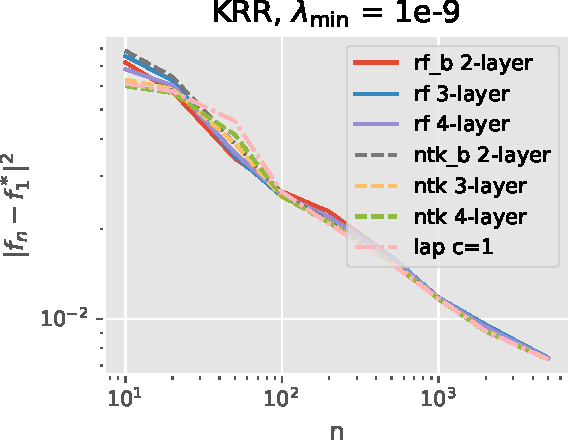
\includegraphics[width=.32\textwidth]{figures/full_kernel_9.pdf}
	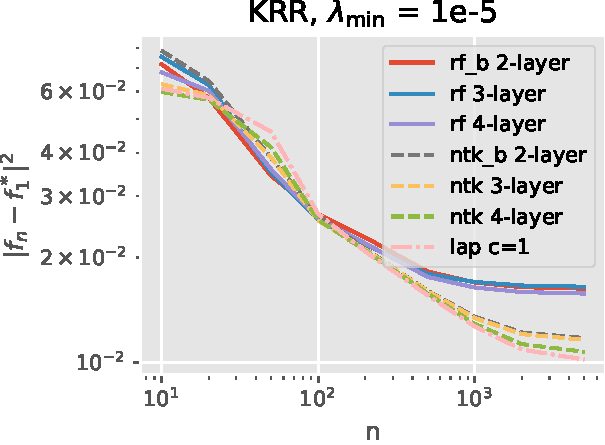
\includegraphics[width=.343\textwidth]{figures/full_kernel_5.pdf}
	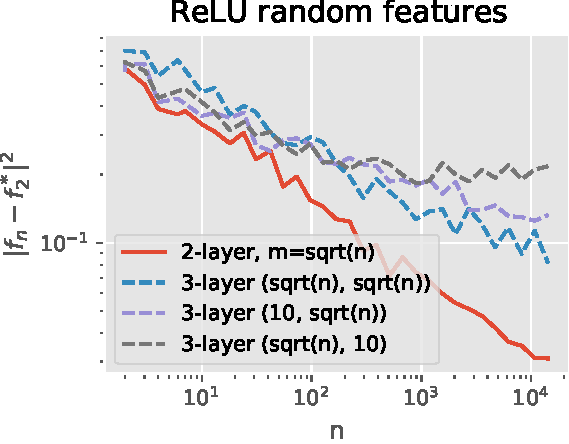
\includegraphics[width=.32\textwidth]{figures/relu_rf.pdf}
	\caption{(left, middle) expected squared error vs sample size~$n$ for kernel ridge regression estimators with different kernels on~$f_1^*$ and with two different budgets on optimization difficulty~$\lambda_{\min}$ (the minimum regularization parameter allowed). (right) ridge regression with one or two layers of random ReLU features on~$f_2^*$, with different scalings of the number of ``neurons'' at each layer in terms of~$n$.}
	\label{fig:synthetic}
\end{figure}


\paragraph{MNIST and Fashion-MNIST.}
In Table~\ref{tab:mnist_acc}, we consider the image classification datasets MNIST and Fashion-MNIST, which both consist of 60k training and 10k test images of size 28x28 with 10 output classes.
We evaluate one-versus-all classifiers obtained by using kernel ridge regression by setting~$y=0.9$ for the correct label and~$y=-0.1$ otherwise.
We train on random subsets of 50k examples and use the remaining 10k examples for validation.
We find that test accuracy is comparable for different numbers of layers in RF or NTK kernels, with a slightly poorer performance for the two-layer case likely due to parity constraints, in agreement with our theoretical result that the decay is the same for different~$L$.
There is a small decrease in accuracy for growing~$L$, which may reflect changes in the decay constants or numerical errors when composing kernels.
The slightly better performance of RF compared to NTK may suggest that these problems are relatively easy (\eg, the regression function is smooth), so that a faster decay is preferable due to better adaptivity to smoothness.

\begin{table}[t]
\caption{Test accuracies on MNIST (left) and Fashion-MNIST (right) for RF and NTK kernels with varying numbers of layers~$L$.
We use kernel ridge regression on 50k samples, with~$\lambda$ optimized on a validation set of size 10k, and report mean and standard errors across 5 such random splits of the 60k training samples.
For comparison, the Laplace kernel with~$c=1$ yields accuracies $98.39 \pm 0.02$ on MNIST and $90.38 \pm 0.06$ on F-MNIST.}
\label{tab:mnist_acc}
\centering

MNIST \hspace{4cm} F-MNIST
\vspace{0.1cm}
\small

\begin{tabular}{ | c |  c |  c |  }
\hline
L &  RF & NTK \\ \hline
2  & 98.60 $\pm$ 0.03 
 & 98.49 $\pm$ 0.02 
\\ 
3  & 98.67 $\pm$ 0.03 
 & 98.53 $\pm$ 0.02 
\\ 
4  & 98.66 $\pm$ 0.02 
 & 98.49 $\pm$ 0.01 
\\ 
5  & 98.65 $\pm$ 0.04 
 & 98.46 $\pm$ 0.02 
\\ 
\hline
\end{tabular}
~~
\begin{tabular}{ | c |  c |  c |  }
\hline
L &  RF & NTK \\ \hline
2  & 90.75 $\pm$ 0.11 
 & 90.65 $\pm$ 0.07 
\\ 
3  & 90.87 $\pm$ 0.16 
 & 90.62 $\pm$ 0.08 
\\ 
4  & 90.89 $\pm$ 0.13 
 & 90.55 $\pm$ 0.07 
\\ 
5  & 90.88 $\pm$ 0.08 
 & 90.50 $\pm$ 0.05 
\\ 
\hline
\end{tabular}

\end{table}

